\chapter{Исследовательский раздел}

Для проверки работоспособности разработанного драйвера были проведены следующие тесты:

\section{Загрузка модуля}

На рисунке \ref{fig:insmod} показан лог загрузки модуля драйвера.

\begin{figure}[h!btp]
	\centering
	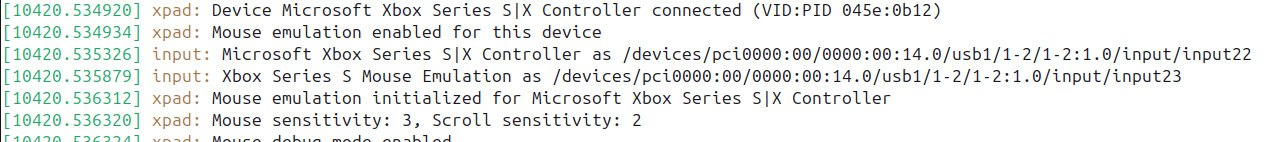
\includegraphics[width=0.7\textwidth]{images/loading.jpg}
	\caption{Загрузка модуля драйвера Xbox Series S}
	\label{fig:insmod}
\end{figure}

При загрузке модуля система выводит сообщение об инициализации драйвера и обнаружении устройства. Драйвер успешно определяет контроллер Xbox Series S, а также параметры.

\section{Тестирование кнопок мыши}

На рисунке \ref{fig:init} показан лог нажатий кнопок контроллера, преобразуемых в события мыши.

\begin{figure}[h!btp]
	\centering
	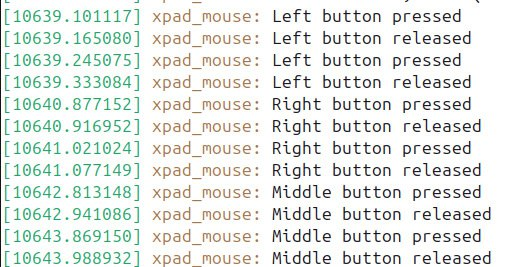
\includegraphics[width=0.5\textwidth]{images/buttons.jpg}
	\caption{Нажатие кнопок мыши (A/B/X)}
	\label{fig:init}
\end{figure}


\section{Тестирование движения курсора}

На рисунке \ref{fig:cursor} показан лог работы курсора при движении левого стика.

\begin{figure}[H]
	\centering
	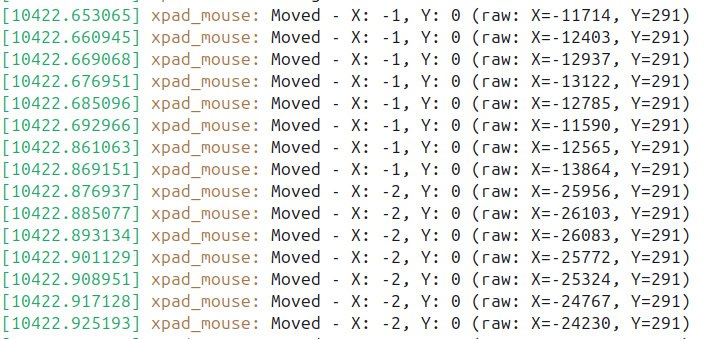
\includegraphics[width=0.5\textwidth]{images/cursor.jpg}
	\caption{Пример работы курсора}
	\label{fig:cursor}
\end{figure}

Движение стиков контроллера преобразуется в относительные движения курсора мыши. Реализована мертвая зона для исключения случайных движений и регулируемая чувствительность.
